\documentclass{beamer}
\usepackage[utf8]{inputenc}
\usepackage[T1]{fontenc}
\usepackage[brazilian]{babel}
\usepackage{lmodern}
\usetheme{default}
\usecolortheme{beaver}
\usepackage{graphicx,xcolor}
\usepackage{amsmath}


\newtheorem{definicao}[theorem]{Definição}
\newtheorem{teorema}[theorem]{Teorema}
\newtheorem{solucao}[theorem]{Solução}
\beamertemplatenavigationsymbolsempty

\makeatletter
\def\th@mystyle{%
	\ttfamily
	\setbeamercolor{block title example}{bg=red!30,fg=black}
	\setbeamercolor{block body example}{bg=red!10,fg=black!80}
	\def\inserttheoremblockenv{exampleblock}
}
\makeatother
\theoremstyle{mystyle}
\newtheorem{algoritmo}[theorem]{Algoritmo}

\title{Raízes (ou Zeros) de Funções Reais}
\author
{
	Prof. Jonathan Esteban Arroyo Silva	
}
\institute
{
	Departamento de Ciência da Computação\\
	Universidade Federal de São João del-Rei\\
	\texttt{silva.jea@ufsj.edu.br}
}
\date{}
\logo{\includegraphics[width=0.2\linewidth]{../ufsj-logo-site}}

\begin{document}
	
\begin{frame}[plain]
    \maketitle
\end{frame}

\begin{frame}[plain]
	\frametitle{Sumário}
	\tableofcontents
\end{frame}

\section{Introdução}

\begin{frame}
	\frametitle{Introdução}
	O problema a seguir:
	\begin{equation*}
		ax^2 + bx + c = 0
	\end{equation*}
	sendo $ a \in \mathbb{R}^{*} $, $ b,c \in \mathbb{R}$, consiste em encontrar os valores de $ x $ para os quais a função:
	\begin{equation*}
		f(x) = ax^2 + bx + c
	\end{equation*}
	seja zero, ou dito de forma simplificada, achar os zeros (ou raízes) da função $ f(x) $
\end{frame}

\begin{frame}
	Afortunadamente, para este tipo de problema a solução é bastante conhecida.
	
	No Brasil é chamada de \textit{fórmula de Bhaskara}:
	\begin{equation*}
		x = \dfrac{-b \pm \sqrt{b^2 - 4ac}}{2a}
	\end{equation*}

	Porém, de modo geral, não podemos encontrar os zeros de uma função através de uma expressão fechada, tendo que recorrer a métodos aproximados.
\end{frame}

\begin{frame}
	Um dos problemas que ocorrem mais frequentemente em trabalhos científicos é o de calcular (ou achar) as raízes de
	equações da forma:
	\begin{equation*}
		f(x) = 0
	\end{equation*}
	sendo $ f(x) $ um polinômio em $ x $ ou uma função transcendente. 
\end{frame}

\begin{frame}
	\frametitle{Exemplo}
	Sendo $ f(x) = x^{2} - 4 \mbox{sen}(x) = 0 $, visualmente é possível dizer onde estão localizadas as raízes
	\begin{figure}
		\centering
		\includegraphics[width=0.6\linewidth]{Figuras/grafico_01}
		\label{fig:grafico01}
	\end{figure}
\end{frame}

\begin{frame}
	\frametitle{Curiosidade}
	No caso vetorial onde $ \mathbf{f} : \mathbb{R}^{n} \rightarrow \mathbb{R}^{n} $, o problema consiste em encontrar o vetor $ \mathbf{x} $ tal que todas as componentes de $ \mathbf{f(x)} $ são iguais a zero simultaneamente.
	\begin{equation*}
		\mathbf{f(x)} = 
		\begin{bmatrix}
			x_{1}^{2} - x_{2}^{2} + 0.2 \\
			- x_{1} + x_{2}^{2} + 0.25
		\end{bmatrix}
		=
		\begin{bmatrix}
			0\\
			0
		\end{bmatrix}
	\end{equation*}
	\pause
	O vetor solução é dado por $ \mathbf{x} = [0.5\;\; 0.5]^{T} $
\end{frame}

\begin{frame}
	\begin{definicao} Se $ f : [a, b] \rightarrow \mathbb{R} $ é uma função dada, um ponto $ \bar{x} \in [a, b]  $ é um zero (ou raiz) de $ f $ se $ f (\bar{x}) = 0 $.
	\end{definicao}
	
	\alert{Nesta disciplina iremos trabalhar apenas com as raízes reais}.
	
	\begin{definicao} Um ponto $ \bar{x} \in [a, b]  $ é uma raiz de multiplicidade $ m $ da equação $ f (x) = 0 $ se $ f(\bar{x}) = f^{\prime}(\bar{x}) = \ldots = f^{(m-1)}(\bar{x}) = 0 $ e $ f^{(m)} (\bar{x}) \neq 0 $.
	\end{definicao}
\end{frame}

\begin{frame}
	\frametitle{Exemplo}
	Sendo $ f(x) = x^{2} + 2x + 1  = (x + 1)^{2} $, a raiz será $ \bar{x} = -1 $ com multiplicidade $ m = 2 $, pois, sendo $ f^{\prime}(x) = 2(x + 1) $, tem-se, $ f(-1) = 0 $, $ f^{\prime}(-1) = 0 $ e $ f^{\prime\prime}(-1) = 2 \neq 0 $
	\begin{figure}
		\centering
		\includegraphics[width=0.6\linewidth]{Figuras/grafico_02}
		\label{fig:grafico02}
	\end{figure}
\end{frame}

\section{Métodos numéricos para achar raízes de funções reais}

\begin{frame}
	\frametitle{Etapas}
	Pode-se dividir o processo de achar as raízes de funções reais em duas partes:
	\begin{itemize}
		\item Isolamento das raízes:
		\begin{itemize}
			\item Encontrar um intervalo $ [a, b] $ que contenha \textbf{apenas uma} raiz
			\item Determinar uma aproximação inicial $ x_{0} $ (ou mais de uma, dependendo do método)
		\end{itemize}
		\item Aplicação do processo iterativo ou refinamento da aproximação:
		\begin{itemize}
			\item Gerar uma sequência $ \{x_{0}, x_{1},\ldots, x_{k}\} $ que convirja para a raiz exata $ \bar{x} $ de $ f (x) = 0 $
		\end{itemize}
	\end{itemize}
\end{frame}

\begin{frame}
	\begin{teorema}
		Se uma função contínua $ f (x) $ assume valores de sinais opostos nos pontos extremos do intervalo $ [a, b] $, isto é, se $ f (a) \cdot f (b) < 0 $, então existe \textbf{pelo menos um} ponto $ \bar{x} \in [a, b] $, tal que	$ f (\bar{x}) = 0 $.		
	\end{teorema}
\end{frame}

\begin{frame}
	\frametitle{Exemplo I}
	Sendo $ f(x) = (x - 1)(x - 2)(x - 3) $, sabemos que existem 3 raízes no intervalo $ [0, 4] $.
	
	É possível ver que no intervalo $  [0.5, 2.5] $ existem duas raízes, porém o Teorema anterior não é aplicável, o que isso significa?	
	\begin{figure}
		\centering
		\includegraphics[width=0.6\linewidth]{Figuras/grafico_03}
		\label{fig:grafico03}
	\end{figure}
\end{frame}

\begin{frame}
	\frametitle{Resposta - Exemplo I}
	Significa apenas que os intervalos utilizados não permitem que utilizemos o Teorema.
	
	Ao definir os intervalos como a seguir:
	\begin{equation*}
		[0.5,1.5]; [1.5,2.5]; [2.5,3.5];
	\end{equation*}
	o Teorema garante que em cada um deles exista \textbf{pelo menos} uma raiz, como observou-se no gráfico.
\end{frame}

\begin{frame}
	\frametitle{Exemplo II}
	Defina um intervalo para achar a raiz positiva (não nula) de $ f(x) = \left( \frac{x}{2} \right)^{2} - \mbox{sen}(x) $
	\begin{figure}
		\centering
		\includegraphics[width=0.6\linewidth]{Figuras/grafico_04}
		\label{fig:grafico04}
	\end{figure}
	\pause
	\textbf{Possível resposta}: $ [1.5,2.5] $
\end{frame}

\begin{frame}
	\frametitle{Exemplo III}
	Encontre um intervalo de tamanho unitário em que haja ao menos uma raiz para $ f(x) = \sqrt{x} - 5 e^{-x} = 0 $ de modo que $ x \geq 0 $
	\pause

	A partir da seguinte tabela:
	\begin{table}
		\centering
		\begin{tabular}{c|c|c}
			x & $f(x)$ & sinal \\
			\hline
			\hline
			0 & -5.0 & <0 \\
			1.0 &  -0.839397205857 & <0 \\
			2.0 & 0.73753714619	& >0 
		\end{tabular}
	\end{table}
	é possível ver que, sendo $ f (x) $ contínua no intervalo $ [1, 2] $, pelo Teorema há ao menos uma raiz.	
\end{frame}

\begin{frame}
	\begin{teorema}
		Sob as hipóteses do teorema anterior, se $ f^{\prime} (x) $ existir e preservar o sinal em $ [a, b] $, então o intervalo contém um único zero de $ f (x) $.
	\end{teorema}
	\begin{figure}
		\centering
		\includegraphics[width=0.45\linewidth]{Figuras/grafico_05a}
		\includegraphics[width=0.45\linewidth]{Figuras/grafico_05b}
		\includegraphics[width=0.45\linewidth]{Figuras/grafico_05c}
		\label{fig:grafico05abc}
	\end{figure}	
\end{frame}

\begin{frame}
	\frametitle{Exemplo}
	É possível garantir que exista apenas uma raiz para a função $ f(x) = \sqrt{x} - 5e^{-x} = 0 $ no intervalo $ [1, 2] $?
	\pause
	
	\textbf{Resposta}: Sim, pois $ f(x) $ é \textbf{contínua} nesse intervalo, $ \mathbf{f(1)\cdot f(2) < 0} $ e $ f^{\prime}(x) = \frac{1}{2\sqrt{x}} + 5e^{-x} > 0, \forall x > 0 $, ou seja, $ f^{\prime} (x) $ \textbf{existe e preserva o sinal}.
\end{frame}

\begin{frame}
	Com esse segundo Teorema, temos as ferramentas suficientes para realizar a primeira parte do processo de achar as raízes de funções reais que é o \textbf{Isolamento das raízes}:
	\begin{itemize}
		\item Encontrar um intervalo $ [a, b] $ que contenha \textbf{apenas uma} raiz
		\item Determinar uma aproximação inicial $ x_{0} $ (ou mais de uma, dependendo do método)
	\end{itemize}
\end{frame}

\section{Método da Bisseção}

\begin{frame}
	\frametitle{Método da Bisseção}
	Pelo primeiro Teorema, se $ f(x) $ tem sinais opostos em $ x = a $ e $ x = b $, então $ f(x) $ tem  no mínimo uma raiz em $ [a,b] $, no método da bisseção é feito o seguinte procedimento:
	\begin{itemize}
		\item Calcula-se o ponto médio do intervalo: $ x_{1} = \dfrac{a + b}{2} $
		\item Se $ f(a) \cdot f(x_{1}) < 0 $, então $ f(x) $ tem uma raiz em $ [a, x_{1}] $, pelo que repetimos o procedimento neste novo intervalo
		\item Se $ f(a) \cdot f(x_{1}) > 0 $, então $ f(x) $ tem uma raiz em $ [x_{1}, b] $, uma vez que $ f(a) $ e $ f(b) $ tem sinais opostos, e repetimos o procedimento neste novo intervalo
	\end{itemize} 
\end{frame}

\begin{frame}
	\begin{algoritmo}
		Para \texttt{k = 1, 2,\ldots, }faça:\\
		\quad x$_{\texttt{k}} \leftarrow$ (a + b)/2\\
		\quad Se f(a)$ \cdot $f(x$ _{\texttt{k}} $) < 0 então:\\
		\quad \quad b $ \leftarrow $ x$ _{\texttt{k}} $\\
		\quad Senão:\\
		\quad \quad a $ \leftarrow $ x$ _{\texttt{k}} $
	\end{algoritmo}
\end{frame}

\begin{frame}
	\frametitle{Exemplo I}
	Aplicando o método para $ f(x) = \sqrt{x} - 5e^{-x} = 0 $ no intervalo $ [1, 2] $ com alguns passos iterativos temos a tabela a seguir:
	\begin{table}
		\centering
		\begin{tabular}{c|c|c||c|c}
			k & a & b & $ x_{k} $ & $f(x)$ \\
			\hline
			\hline
			1 & 1.0 & 2.0 & 1.5 & 0.10909407064943988 \\
			2 & 1.0      & 1.5    & 1.25      & -0.3144899955510556    \\ 
			3 & 1.25     & 1.5    & 1.375     & -0.09159403906787489   \\
			4 & 1.375    & 1.5    & 1.4375    &  0.011353785350889156  \\
			5 & 1.375    & 1.4375 & 1.40625   & -0.039448573664487174  \\
			6 & 1.40625  & 1.4375 & 1.421875  & -0.013882136918039523  \\
			7 & 1.421875 & 1.4375 & 1.4296875 & -0.0012231854840827339 \\ 
		\end{tabular}
	\end{table}
\end{frame}

\begin{frame}
	\frametitle{Exemplo II}
	\centering
	\href{https://colab.research.google.com/drive/16A79ot1vYg77thZVmoFotmrI4zaSPcOA?usp=sharing}{\beamergotobutton{Link para exemplo interativo}}
	
\end{frame}

\section{Critério de parada e Ordem de convergência}

\begin{frame}
	\frametitle{Critério de parada}
	Na prática a sequência de soluções aproximadas é interrompida quando seus valores satisfizerem a pelo menos um dos seguintes critérios:
	\begin{gather*}
		\left| x_{k} - x_{k - 1}\right| \leq \epsilon \text{ (Erro absoluto)}\\
		\left| \frac{x_{k} - x_{k - 1}}{x_{k}}\right|  \leq \epsilon \text{ (Erro relativo)}\\
		|f(x_{k})| \leq \epsilon
	\end{gather*}
	sendo $ \epsilon $ a precisão ou tolerância \textit{fornecida} como parâmetro para o processo iterativo.
\end{frame}

\begin{frame}
	\frametitle{Critério de parada - observações}
	\begin{itemize}
		\item É importante sempre limitar a quantidade de iterações, ou seja, fornecer um $ k_{\mbox{final}} $ ou $ k_{\mbox{maximo}} $
		\item Em relação à precisão fornecida, normalmente tomamos $ \epsilon = 10^{-m} $ onde $ m $ é o número de casas decimais que queremos corretas no resultado
		\item A utilização do erro relativo é o mais adequado dentre os três citados acima
	\end{itemize} 	
\end{frame}

\begin{frame}
	\frametitle{Ordem de convergência}
	Um indicador importante sobre o \textit{desempenho} do método é a rapidez da sequência de aproximações $ \{x_{0}, x_{1},\ldots, x_{k}\} $ em convergir para a raiz exata $ \bar{x} $
	\begin{definicao}
		Uma sequência $ \{x_{k}| k \geq 0\} $ é dita convergir com ordem $ p \geq 1 $ para um ponto $ \bar{x} $ se:
		\begin{equation*}
			|\bar{x} - x_{k}| \leq c |\bar{x} - x_{k - 1}|^{p},\;\; k \geq 0  
		\end{equation*}
		para uma constante $ c > 0 $
	\end{definicao}
\end{frame}

\begin{frame}
	\frametitle{Ordem de convergência - observações}
	Sendo $ c < 1 $, dizemos que:
	\begin{itemize}
		\item se $ p = 1 $ a convergência é linear
		\item se 1 < p < 2 a convergência é super-linear
		\item se p = 2 a convergência é quadrática
	\end{itemize} 
\end{frame}

\section{Método do ponto fixo}

\begin{frame}
	\frametitle{Problemas de ponto fixo}
	Antes de falar do próximo método numérico, é necessário apresentar alguns conceitos:
	\begin{definicao}
		O \textbf{ponto fixo} de uma determinada função $ g: \mathbb{R} \rightarrow \mathbb{R} $ é o valor $ x $ que satisfaz: 
		\begin{equation*}
			x = g(x)
		\end{equation*}
	\end{definicao}
\end{frame}

\begin{frame}
	\frametitle{Problemas de ponto fixo - observações}
	\begin{itemize}
		\item Muitos métodos iterativos para resolver este tipo de problema utilizam uma função de iteração da forma:
		\begin{equation*}
			x_{k} = g(x_{k-1})
		\end{equation*}
		sendo que os pontos fixos de $ g $ também são solução para a equação $ f (x) = 0 $		 
		\item Para uma determinada equação $ f (x) = 0 $, pode existir mais de um problema de ponto fixo equivalente $ x = g(x) $ com distintos $ g $
	\end{itemize} 
\end{frame}

\begin{frame}
	\frametitle{Exemplo}
	Dado $ f (x) = x^{2} - x - 2 $, é equivalentes resolver $ f (x) = 0 $ a resolver os seguinte problemas de ponto fixo:
	\begin{itemize}
		\item $g(x) = x^{2} - 2 $
		\item $g(x) = \sqrt{x + 2} $
		\item $g(x) = 1 + 2/x $
		\item $g(x) = \dfrac{x^{2} + 2}{2x - 1} $		
	\end{itemize}
	\pause
	\alert{Entretanto nem todas estas expressões são adequadas para uma função de iteração}
\end{frame}

\begin{frame}
	\frametitle{Convergência do método de ponto fixo}
	Para que um problema de ponto fixo $ x = g(x) $, seja adequado para a aplicação de métodos iterativos, ele precisa satisfazer os seguintes critérios: 
	\begin{itemize}
		\item $ g(x) $ e $ g^{\prime}(x) $ devem ser continuas num intervalo $ I $ contendo a raiz procurada
		\item $ |g^{\prime}(x)| < 1, \forall x \in I $
	\end{itemize} 
\end{frame}

\begin{frame}
	\frametitle{Método do ponto fixo}
	Após definir uma função de iteração $ g(x) $, uma aproximação inicial adequada $ x_{0} $ (no intervalo $ I $), a precisão $ \epsilon $ e o numero máximo de iterações $ k_{\text{max}} $:
	\begin{algoritmo}
		\# Inicializar a variável\\
		 k $\leftarrow$ 1\\ 
		Enquanto o \textbf{critério de parada não for satisfeito}, faça:\\
		\quad x$ _{\texttt{k}} \leftarrow $ g(x$ _{\texttt{k-1}}$) \\
		\quad k $\leftarrow$ k + 1
	\end{algoritmo}
\end{frame}

\begin{frame}
	\frametitle{Exemplo I}
	Dado $ f (x) = x^{2} - x - 2 $, considerando $ I = [1.5, 2.5] $ (uma vez que a raiz exata é $ \bar{x} = 2.0 $), verifique se a função de iteração $ g(x) = x^{2} - 2 $, satisfaz os critérios de convergência do método do ponto fixo.
	\pause
	
	\begin{itemize}
		\item Uma vez que $ g^{\prime}(x) = 2x $, sabemos que $ g(x) $ e $ g^{\prime}(x) $ são contínuas em $ I $
		\item Porém $ \max_{x \in I}|2x| > 1 $, logo, o método do ponto fixo \alert{não converge} para essa escolha da função de iteração
	\end{itemize}
\end{frame}

\begin{frame}
	\frametitle{Exemplo II}
	Verifique se a função de iteração $ g(x) = \sqrt{x + 2} $, satisfaz os critérios de convergência do método do ponto fixo do problema anterior.
	\pause
	
	\begin{itemize}
		\item Uma vez que $ g^{\prime}(x) = \dfrac{1}{2\sqrt{x + 2}} $, sabemos que $ g(x) $ e $ g^{\prime}(x) $ são contínuas em $ I $
		\item Como $ \max_{x \in I} \left| \dfrac{1}{2\sqrt{x + 2}} \right| = 0.267 < 1 $, logo, o método do ponto fixo \alert{converge} para essa escolha da função de iteração
	\end{itemize}
\end{frame}

\begin{frame}
	\frametitle{Exemplo II - Implementação}
	\centering
	\href{https://colab.research.google.com/drive/1Ol4hdP697Brh07Daga9DyhJivxgfXbYK?usp=sharing}{\beamergotobutton{Link para exemplo interativo}}
\end{frame}

\section{Método de Newton}

\begin{frame}
	\frametitle{Método de Newton}
	\begin{itemize}
		\item O método de Newton é obtido utilizando $ g(x) = x - \dfrac{f(x)}{f^{\prime}(x)} $ como função de iteração para o Método de ponto fixo
		\item Possui ordem de convergência igual a 2, em condições ideais
		\item É o método clássico mais utilizado para este tipo de problemas
	\end{itemize}
\end{frame}

\begin{frame}
	\begin{algoritmo}
		\# Inicializar a variável\\
		k $\leftarrow$ 1\\
		Enquanto o \textbf{critério de parada não for satisfeito}, faça:\\
		\quad x$ _{\texttt{k}} \leftarrow$ x$ _{\texttt{k-1}} $ - $ \dfrac{\texttt{f(x}_{\texttt{k-1}} \texttt{)}}{\texttt{f}^{\prime}\texttt{(x}_{\texttt{k-1}} \texttt{)}} $ \\
		\quad k $\leftarrow$ k + 1
	\end{algoritmo}
\end{frame}

\begin{frame}
	\frametitle{Exemplo}
	Resolva $ f (x) = x^{2} - x - 2 = 0 $, considerando $ I = [1.5, 2.5] $.
	\pause
	
	\begin{itemize}
		\item Das informações necessárias para utilizar o método de Newton, falta apenas explicitar que $ f^{\prime}(x) = 2x - 1 $
		\item Tem-se então a fórmula de iteração:
		\begin{equation*}
			x_{k} = x_{k - 1} - \frac{x_{k - 1}^{2} - x_{k - 1} - 2}{2x_{k - 1} - 1}
		\end{equation*}
	\end{itemize}
\end{frame}

\begin{frame}
	\frametitle{Exemplo - Implementação}
	\centering
	\href{https://colab.research.google.com/drive/1OnVWIXh918bJg1vS8VZVvc5EM-MrwY2c?usp=sharing}{\beamergotobutton{Link para exemplo interativo}}
\end{frame}

\section{Método da Secante}

\begin{frame}
	\frametitle{Método da Secante}
	\begin{itemize}
		\item O método da secante é obtido utilizando a aproximação $ f^{\prime}(x_{k - 1}) \approx \frac{f(x_{k - 1}) - f(x_{k - 2})}{x_{k - 1} - x_{k - 2}} $ para a derivada de $ f(x) $ no método de Newton
		\item Possui ordem de convergência super linear
		\item É recomendado quando não se tem uma expressão explícita ou muito complexa para $ f^{\prime}(x) $
	\end{itemize}	
\end{frame}

\begin{frame}
	\begin{algoritmo}
		\# Inicializar a variável\\
		k $\leftarrow$ 1 \\
		Enquanto o \textbf{critério de parada não for satisfeito}, faça:\\
		\quad x$ _{\texttt{k}} \leftarrow \dfrac{x_{k - 2} \cdot f(x_{k - 1}) - x_{k - 1} \cdot f(x_{k - 2})}{f(x_{k - 1}) - f(x_{k - 2}) } $ \\
		\quad k $\leftarrow$ k + 1
	\end{algoritmo}
\end{frame}

\begin{frame}
	\frametitle{Exemplo}
	Resolva $ f (x) = x^{2} - x - 2 = 0 $, considerando $ I = [1.5, 2.5] $.
	\pause
	
	\begin{itemize}
		\item A fórmula de iteração é dada por:
		\begin{equation*}
			x_{k} =\frac{x_{k - 2} \cdot (x_{k - 1}^{2} - x_{k - 1} - 2) - x_{k - 1} \cdot (x_{k- 2}^{2} - x_{k - 2} - 2)}{(x_{k - 1}^{2} - x_{k - 1} - 2) - (x_{k - 2}^{2} - x_{k - 2} - 2)}
		\end{equation*}
	\end{itemize}
\end{frame}

\begin{frame}
	\frametitle{Exemplo - Implementação}
	\centering
	\href{https://colab.research.google.com/drive/1vZgdMgXO5qvClp5dK3kR-Qs4BnWPkcu2?usp=sharing}{\beamergotobutton{Link para exemplo interativo}}
\end{frame}

\begin{frame}
	\frametitle{Conclusão I}	
	Foram abordados os seguintes assuntos:
	\begin{itemize}
		\item Apresentação do problema de achar raízes de funções reais
		\item As etapas para a aplicação dos métodos numéricos
		\begin{itemize}
			\item Isolamento das raízes
			\item Aplicação do processo iterativo
		\end{itemize}
		\item O método da Bisseção
		\item Apresentação dos conceitos de Critério de parada e Ordem de convergência
	\end{itemize}
\end{frame}

\begin{frame}
	\frametitle{Conclusão II}	
	\begin{itemize}
		\item O método do ponto fixo
		\item O método de Newton
		\item O método da Secante
	\end{itemize}
\end{frame}

\begin{frame}[plain]
\bigskip
\bigskip
\bigskip
\bigskip
\bigskip
\begin{figure}
	\centering
	
\includegraphics[width=0.9\linewidth]{../Luffy_v}
	\label{fig:luffyv}
\end{figure}
\end{frame}

\end{document}
